% Figure -- the locator's implementation flow as firmware (English twin of fig-pipeline.tex).
%
% Build with:  pdflatex fig-pipeline-en.tex
% Produces fig-pipeline-en.pdf, included in report.tex.
%
% Same conventions and palette as the thesis flowchart (fluxograma-metodologia.tex):
%   - plain arrow between boxes ........ the next stage works on the previous one's output;
%   - fork / join bar .................. branches work on the SAME input and are then
%                                        combined (run one after another on the single-core
%                                        microcontroller).

\documentclass[border=4pt]{standalone}

\usepackage[T1]{fontenc}
\usepackage[utf8]{inputenc}
\usepackage[english]{babel}
\usepackage{lmodern}
\usepackage{tikz}
\usetikzlibrary{arrows.meta}

\definecolor{cxfill}{HTML}{BEE3F0}
\definecolor{cxline}{HTML}{1F5C7A}
\definecolor{bdfill}{HTML}{F4F9FC}
\definecolor{bdline}{HTML}{8FB3C6}
\definecolor{rsfill}{HTML}{7FC3DC}
\definecolor{ntcolor}{HTML}{3C6A82}

\begin{document}
\sffamily
\hyphenpenalty=10000 \exhyphenpenalty=10000
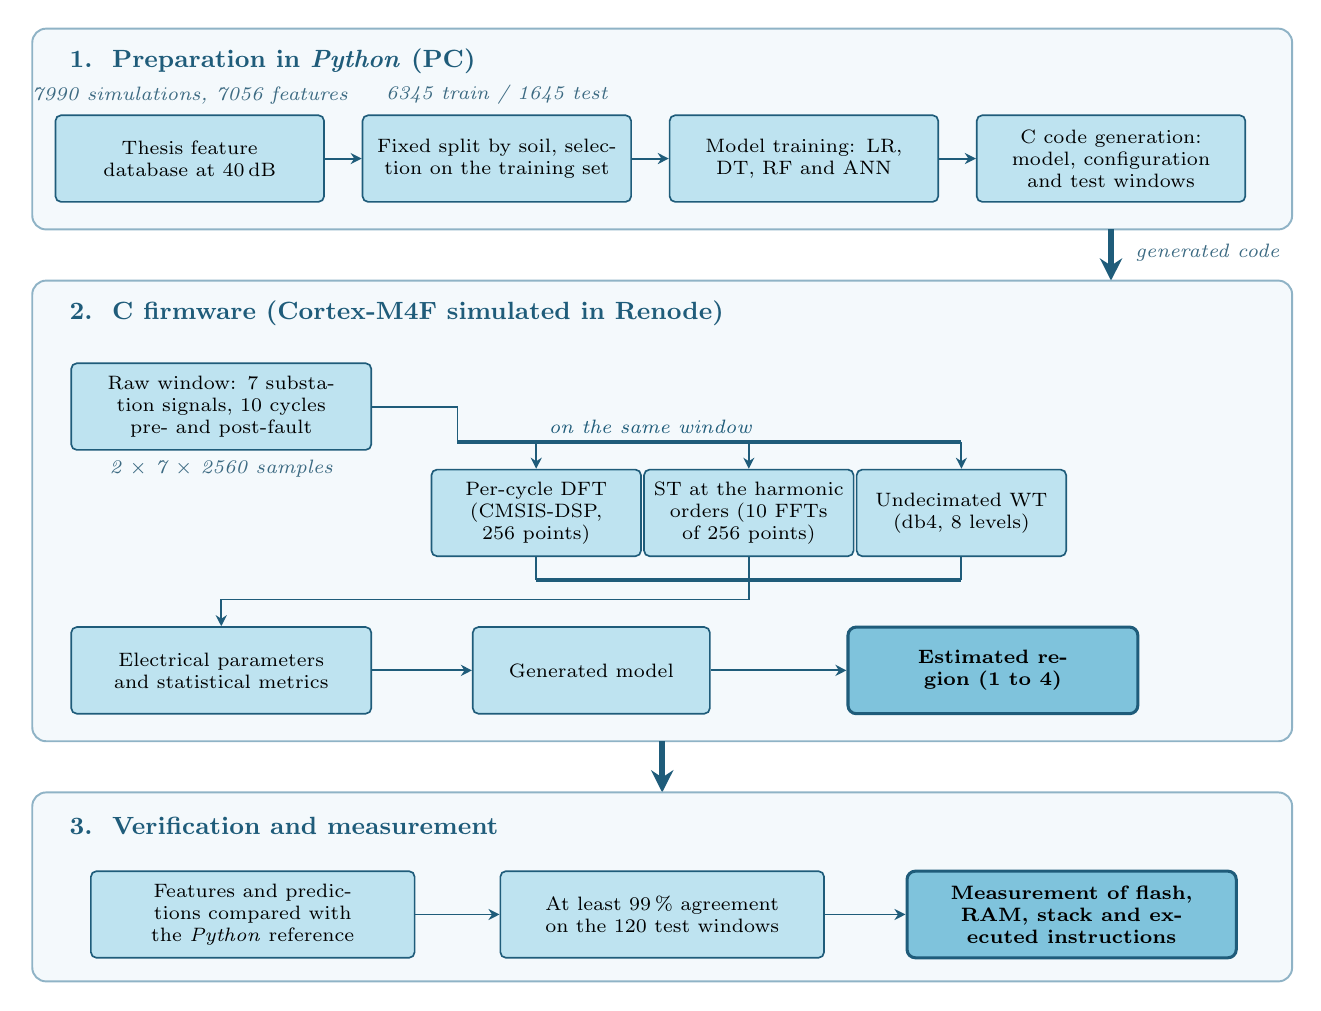
\begin{tikzpicture}[
  x=1cm, y=1cm,
  etapa/.style={
    rounded corners=2pt, draw=cxline, fill=cxfill, line width=0.6pt,
    text width=#1, align=center, inner sep=3pt, minimum height=1.10cm,
    font=\scriptsize},
  etapa/.default=3.20cm,
  resultado/.style={
    rounded corners=3pt, draw=cxline, fill=rsfill, line width=1.1pt,
    text width=#1, align=center, inner sep=4pt, minimum height=1.10cm,
    font=\scriptsize\bfseries},
  resultado/.default=3.20cm,
  faixa/.style={rounded corners=5pt, draw=bdline, fill=bdfill, line width=0.7pt},
  titulo/.style={font=\small\bfseries, text=cxline},
  seta/.style={-{Stealth[length=4pt,width=4pt]}, draw=cxline, line width=0.7pt},
  liga/.style={draw=cxline, line width=0.7pt},
  setona/.style={-{Stealth[length=8pt,width=8pt]}, draw=cxline, line width=2pt},
  tracejada/.style={-{Stealth[length=4pt,width=4pt]}, draw=cxline, line width=0.7pt,
                    dash pattern=on 3pt off 2pt},
  barra/.style={draw=cxline, line width=1.6pt},
  nota/.style={font=\scriptsize\itshape, text=ntcolor, inner sep=1.5pt},
  par/.style={font=\scriptsize\itshape, text=cxline, inner sep=1.5pt},
]

% ===================== BAND 1 -- preparation in Python =====================
\fill[faixa] (0.2,-0.2) rectangle (16.2,-2.75);
\node[titulo, anchor=west] at (0.55,-0.62) {1.\ \ Preparation in \textit{Python} (PC)};

\node[etapa] (a1) at (2.2,-1.85) {Thesis feature database at 40\,dB};
\node[etapa] (a2) at (6.1,-1.85) {Fixed split by soil, selection on the training set};
\node[etapa] (a3) at (10.0,-1.85) {Model training: LR, DT, RF and ANN};
\node[etapa] (a4) at (13.9,-1.85) {C code generation: model, configuration and test windows};

\draw[seta] (a1) -- (a2);
\draw[seta] (a2) -- (a3);
\draw[seta] (a3) -- (a4);
\node[nota, above] at (2.2,-1.22) {7990 simulations, 7056 features};
\node[nota, above] at (6.1,-1.22) {6345 train / 1645 test};

\draw[setona] (13.9,-2.75) -- (13.9,-3.40);
\node[nota, anchor=west] at (14.15,-3.05) {generated code};

% ===================== BAND 2 -- firmware ===================
\fill[faixa] (0.2,-3.40) rectangle (16.2,-9.25);
\node[titulo, anchor=west] at (0.55,-3.82) {2.\ \ C firmware (Cortex-M4F simulated in Renode)};

\node[etapa=3.6cm] (b1) at (2.6,-5.00)
  {Raw window: 7 substation signals, 10 cycles pre- and post-fault};
\node[nota, below] at (2.6,-5.62) {2 $\times$ 7 $\times$ 2560 samples};

% fork: the three transforms work on the SAME window
\draw[liga] (b1.east) -- (5.6,-5.00) -- (5.6,-5.45);
\draw[barra] (5.6,-5.45) -- (12.0,-5.45);
\node[par, anchor=west] at (6.7,-5.26) {on the same window};

\node[etapa=2.45cm] (b2) at (6.6,-6.35) {Per-cycle DFT (CMSIS-DSP, 256 points)};
\node[etapa=2.45cm] (b3) at (9.3,-6.35) {ST at the harmonic orders (10 FFTs of 256 points)};
\node[etapa=2.45cm] (b4) at (12.0,-6.35) {Undecimated WT (db4, 8 levels)};
\draw[seta] (6.6,-5.45) -- (b2.north);
\draw[seta] (9.3,-5.45) -- (b3.north);
\draw[seta] (12.0,-5.45) -- (b4.north);

% join
\draw[liga] (b2.south) -- (6.6,-7.20);
\draw[liga] (b3.south) -- (9.3,-7.20);
\draw[liga] (b4.south) -- (12.0,-7.20);
\draw[barra] (6.6,-7.20) -- (12.0,-7.20);

\node[etapa=3.6cm] (b5) at (2.6,-8.35) {Electrical parameters and statistical metrics};
\draw[seta] (9.3,-7.20) -- (9.3,-7.45) -- (2.6,-7.45) -- (b5.north);
\node[etapa=2.8cm] (b6) at (7.3,-8.35) {Generated model};
\node[resultado=3.4cm] (b7) at (12.4,-8.35) {Estimated region (1 to 4)};
\draw[seta] (b5) -- (b6);
\draw[seta] (b6) -- (b7);

\draw[setona] (8.2,-9.25) -- (8.2,-9.90);

% ===================== BAND 3 -- verification and measurement ===================
\fill[faixa] (0.2,-9.90) rectangle (16.2,-12.30);
\node[titulo, anchor=west] at (0.55,-10.32) {3.\ \ Verification and measurement};

\node[etapa=3.9cm] (c1) at (3.0,-11.45)
  {Features and predictions compared with the \textit{Python} reference};
\node[etapa=3.9cm] (c2) at (8.2,-11.45)
  {At least 99\,\% agreement on the 120 test windows};
\node[resultado=3.9cm] (c3) at (13.4,-11.45)
  {Measurement of flash, RAM, stack and executed instructions};
\draw[seta] (c1) -- (c2);
\draw[seta] (c2) -- (c3);

\end{tikzpicture}
\end{document}
